	%----------------------------------------------------------------------------------------
%	PACKAGES AND OTHER DOCUMENT CONFIGURATIONS
%----------------------------------------------------------------------------------------

\documentclass[a4paper,11pt]{kth-mag}
\usepackage[T1]{fontenc}
\usepackage{textcomp}
\usepackage{lmodern}
\usepackage[utf8]{inputenc}
\usepackage[swedish,english]{babel}
\usepackage{modifications}
\usepackage{mathtools} 
\usepackage{hyperref}
\usepackage{booktabs}
\usepackage{multirow}
\usepackage{pgfplots}
\usepackage{float}
\usepackage{graphicx}
\usepackage{caption}
\usepackage{subcaption}
\usepackage{tabularx}
\DeclareUnicodeCharacter{00A0}{ }

%----------------------------------------------------------------------------------------
%	TITLE PAGE
%----------------------------------------------------------------------------------------

\title{Automatic Package Measuring}

\subtitle{Measuring the dimensions of cuboid objects with a single, uncalibrated view}
\foreigntitle{Automatisk paketmätning}
\author{Tobias Andersson\\\MakeLowercase{tobias2@kth.se}}
\date{June 2015}
\blurb{Master’s Thesis in Computer Science (30 credits)\\Supervisor: Mårten Björkman (celle@csc.kth.se)\\Examiner: Danica Kragic (dani@kth.se)\\~\\Project provider:\\Roland Persson (roland.persson@bontouch.com)\\Bontouch AB}
\trita{}
\begin{document}
\frontmatter
\pagestyle{empty}
\removepagenumbers
\maketitle
\selectlanguage{english}

%----------------------------------------------------------------------------------------
%	ABSTRACT + TABLE OF CONTENTS
%----------------------------------------------------------------------------------------

\begin{abstract}
%Suppose that one needs to know the dimensions of a package, but does not have a measuring tool.
%What most people do have is a smartphone, which has the potential to be a measuring tool.
%If a reference object of known size is placed on top of the package, and the two objects are filmed together, the dimensions of the package can be calculated.

This report presents a method to measure the dimensions of cuboid packages automatically with a single uncalibrated view.
The method was designed to be used on a mobile device, and considers the consequent hardware and time constraints.

The method uses a planar reference object of known size, which is placed on top of the package.
The reference object and package are detected automatically in the image, and their positions are fed to a measuring algorithm.

The measuring algorithm uses the geometry of cuboids to avoid prior camera calibration.
By using the vanishing points which are induced by the edges of the package, the camera can be calibrated online from a single view.

With this method, a correct measurement was achieved in $92\%$ of the images when a subset of the tested camera poses were used. On the complete test set the success rate was $51\%$.
Online testing on a smartphone shows that the detection algorithm is not yet mature to be run in a real-time application, but could work well in a non-real time application.

%A version of the algorithm which used calibrated views were also implemented, to determine how much performance needed to be sacrificed to gain the convenience of not having to go through the calibration procedure.
%The success rates when testing the measuring algorithm in isolation was $81\%$ for uncalibrated views, and $93\%$ for calibrated views.

\end{abstract}
\clearpage

\begin{foreignabstract}{swedish}
Att göra % TODO abstract
\end{foreignabstract}

\clearpage
\tableofcontents*
\mainmatter
\pagestyle{newchap}

%----------------------------------------------------------------------------------------
%	ESSAY BODY
%----------------------------------------------------------------------------------------

Computer vision applications on handheld devices is an area which has received growing interest in recent years. 
Modern smartphones are cheap, and their cameras are good enough for most computer vision purposes.
% TODO hitta källa som säger nåt intressant om detta

An interesting computer vision problem, which can be useful in a smartphone is to measure the dimensions of an object, a postal package, for example.
Imagine that you would like to know the dimensions of a package, but don't have a measuring tool.
Since almost everyone carries a smartphone with them, a practical solution would be to have an app which can measure the package, without measuring tape or ruler.
If a reference object, like a credit card for example, is placed on top of the package, it should be possible to measure its dimensions by filming the package and reference object together.

\section{Problem Statement}\label{problem-statement}
In order for a measuring solution like the one described above, to be useful, it must be easy to use. % commas correct?
The measuring process should therefore not require any user intervention, such as marking the reference object or package in the image, they will be detected automatically by the program.

Computer vision applications which aim to extract metric information from a scene typically require knowledge about the camera's properties, and position.
Gathering the necessary information about the camera should therefore not require any additional steps, such as calibrating the camera beforehand.
I.e. the problem is to be solved using an \textit{uncalibrated view}.
To further simplify the process, and to reduce computational complexity, the problem should be solved using only one, uncalibrated view.

However, because a calibrated view is expected to result in higher accuracy, it would be interesting to compare the performance two methods.

For this approach to be successful, two components must exist, and work reasonably well: the detection process, and the measuring process.
The detection process consists of finding the position of the reference object and the package in the image, and the measuring process consists of using their positions to calculate the dimensions of the package.

To assess the quality of the result, the two components should be evaluated both separately, and together. 
Each of the three categories will be tested for \textit{robustness} and \textit{accuracy}.
Robustness is defined to be rate at which the result is reasonably correct.
Accuracy is defined to be how accurate the result is when a reasonable solution is found.

In principle all of the above can be tested offline, using pictures taken with a smartphone.
This will be the method used when evaluating the result
However, since the purpose of the program is to be used in a smartphone, it will also be embedded in a smartphone demo app, to show that it performs well enough in its intended environment, and more importantly, that the program is fast enough to be used in a smartphone.

\section{Delimitations} % limiatations delimitations?
In an finished consumer smartphone application, it would be desirable to have the option to choose between a multitude of reference objects, like credit cards, matchboxes, smartphones, papers, and more. 
To simplify the detection process, only white papers from the ISO 216 A-series (e.g. A4) will be considered in this thesis.
The reason behind this choice is that papers of this type are very common, and easy to detect.

The type of packages considered are limited to packages with a cuboid shape, and with a colour that has reasonable contrast to that of the reference object.

The package must stand on a flat surface, and there the area in close proximity to the package should be empty.

% TODO Section about Bontouch/Postnord???
In this chapter related work will be presented.
% TODO Other reports have this before background. A) Why? B) probably best to follow the convention
In this chapter the theoretical concepts used throughout the report is presented. Knowledge of three computer vision related fields is necessary to understand the following chapters. These are projective geometry, image processing, and image analysis.

\section{Projective geometry}
Everyone has a basic understanding of what projective geometry is, and how it works.
We experience it at every wake moment, without thinking about it. 
Based on where one is standing and when looking at a shape, the shape can look very different. % TODO ändra
Projective geometry describes these kinds of phenomena.
In this section some basic concepts in projective geometry is presented, and how images are formed in cameras.

At first glance it seems that very little is preserved by a projective transformation, or "changing perspective" in informal term.
Neither shape, lengths, angles, distances, or ratios of distances are preserved.
The most general property in a scene that is preserved by a projective transformation is straightness. \cite[1]{hartley-zisserman}

In euclidean geometry, a point in two-dimensional space is typically represented by cartesian coordinates, a pair of numbers, which represent the distance to the origin in each dimension. % TODO rephrase
In projective geometry homogeneous coordinates are used instead.
To convert the cartesian coordinate pair $(x,y)$ to homogeneous coordinates, a one is appended to the cartesian coordinates, resulting in the point $(x,y,1)$. 
An interesting property about homogeneous coordinates is that they ignore scale, meaning that $(x,y,1)$ and $(kx,ky,k)$ represents the same point for any nonzero value $k$.
To convert back to cartesian coordinates, divide by $k$ and remove the $1$.\cite[2]{hartley-zisserman} % Rephrase this part

\subsection{Camera Model}\label{camera-model}
Cameras, create a 2D representation of a 3D world.
The camera model used in this thesis is called the projective camera model.
It is based on a pinhole camera model, where all rays of light pass through a single point called the camera centre, $C$. Before reaching $C$, each ray will pierce the image plane, where the image is projected.
It's location is determined by $f$, the focal length of the camera.

\begin{figure}[h]
\begin{center}
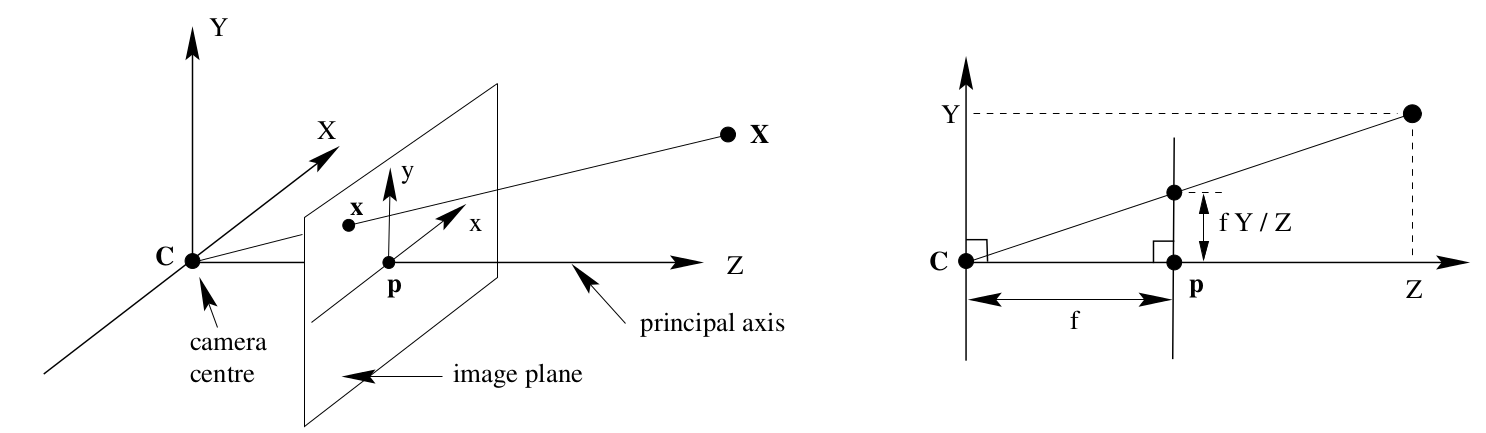
\includegraphics[width=0.6\textwidth]{figures/central_projection_camera.png}
\end{center}
\caption{The central projection camera model. The world and image coordinate systems are aligned. The image plane centred on the $Z$ axis, length $f$ in front of the origin.}
\label{fig:central_projection_camera} % TODO hur referera? zisserman-hartley s.154
\end{figure}

Using the central projection model, as shown in figure \ref{fig:central_projection_camera}, a 3D point can be mapped to a 2D image point, as follows: $(X,Y,Z)^T\mapsto(fX/Z,fY/Z)^T$.
The central projection model makes some rather limiting assumptions, which, which we will now generalise.
First, the origin of the image coordinate system is normally not in the centre.
In that case an offset to the principal point, $(p_{x}, p_{y})$, is added, which represents the coordinates of the centre of the image.
Furthermore, the mapping above assumes that the camera is not rotated, and located in the origin of the world coordinate system. Taking this into account, the following equation can be formed:
\begin{equation}\label{eq:projection1}
\begin{pmatrix}	\tilde{u}\\\tilde{v}\\\tilde{w}\end{pmatrix} = 
\begin{pmatrix}
	f & 0 & p_{x} & 0\\
	0 & f & p_{y} & 0\\
	0 & 0 & 1 & 0
\end{pmatrix}
\begin{pmatrix}
	r_{11} & r_{12} & r_{13} & t_{1}\\
	r_{21} & r_{22} & r_{23} & t_{2}\\
	r_{31} & r_{32} & r_{33} & t_{3}
\end{pmatrix}
\begin{pmatrix}	X\\Y\\Z\\1\end{pmatrix}
\end{equation}

where $(\tilde{x},\tilde{y},\tilde{z})^T$ are the homogeneous coordinates of the pixel in the image of the world coordinates $(X,Y,Z)$.
As explained earlier, the cartesian coordinates are obtained by dividing by $\tilde{w}$:
$$
u = \frac{\tilde{u}}{\tilde{w}},~~v = \frac{\tilde{v}}{\tilde{w}}
$$
The above is the projective camera model that will be used in this thesis. 
It can be generalised further to take things like pixel skew and non-square pixels into account, but those are rare cases and are therefore left out.

The left of the two matrices above is called the calibration matrix, or intrinsic matrix, $K$.
It contains the intrinsic parameters of the camera.
The intrinsic parameters depend only on the camera, and is always the same for the a given camera, if there is no change in zoom.
The right matrix is called the extrinsic matrix, and contains the extrinsic parameters of the camera.
The extrinsic parameters are not tied to the camera's properties, but instead depend on where in the world the camera is located, and where it points.
The above can also be written in the more concise form $x = K[R|t]X$.

When multiplied together, the intrinsic and extrinsic matrices form a $3\times4$-matrix, called the camera matrix, or the projection matrix, $P$:
\begin{equation} \label{eq:projection2}
\begin{pmatrix} \tilde{u} \\ \tilde{v} \\ \tilde{w} \end{pmatrix} = \lambda
\begin{pmatrix} p_{11} & p_{12} & p_{13} & p_{14} \\
 				p_{21} & p_{22} & p_{23} & p_{24} \\
				p_{31} & p_{32} & p_{33} & p_{34} \end{pmatrix}
\begin{pmatrix}X \\Y \\Z \\1\end{pmatrix}
\end{equation}
It can be determined up to an arbitrary scale factor, $\lambda$.
Because $\lambda$ is arbitrary, $P$ only has 11 degrees of freedom. We can simplify to:
\begin{equation}\label{eq:projection3}
\begin{pmatrix} \tilde{u} \\ \tilde{v} \\ \tilde{w} \end{pmatrix} =
\begin{pmatrix} p_{11} & p_{12} & p_{13} & p_{14} \\
 				p_{21} & p_{22} & p_{23} & p_{24} \\
				p_{31} & p_{32} & p_{33} & 1 \end{pmatrix}
\begin{pmatrix}X \\Y \\Z \\1\end{pmatrix}
\end{equation}
where the scaling of the elements of $P$ is implicit for convenience. \cite[153-165]{hartley-zisserman}

\subsection{Planar Homographies}\label{planar-homographies}

\begin{figure}[h]
\begin{center}
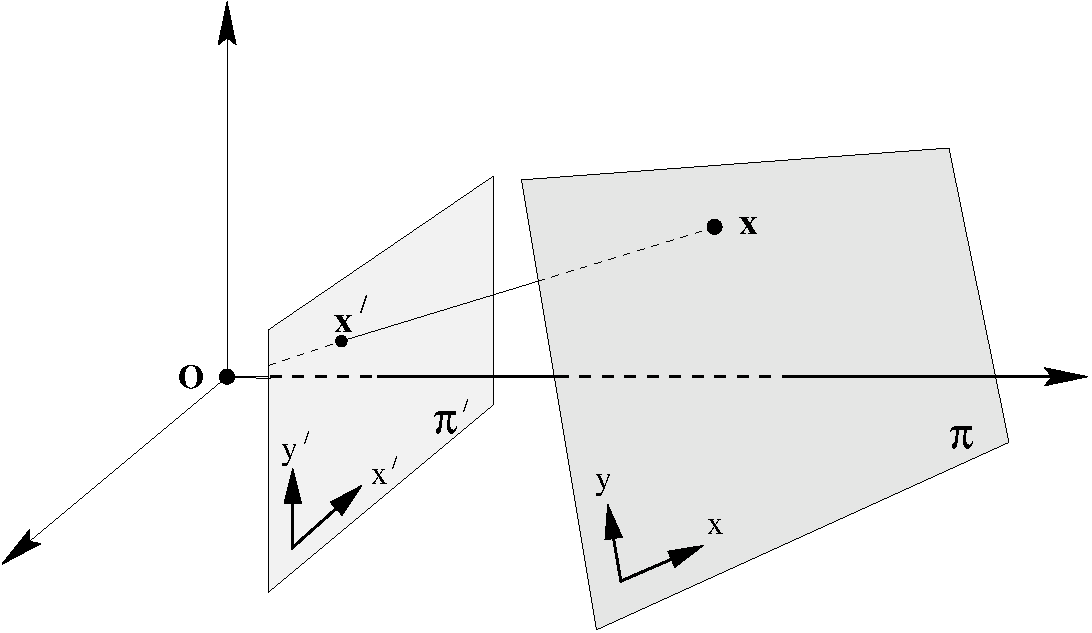
\includegraphics[width=0.6\textwidth]{figures/planar_homography.pdf}
\end{center}
\caption{A point on a plane in the world is projected to the image plane. A planar homography can be used to map points between the two planes} % TODO hur referera? Tagen från hartley-zisserman s. 34
\label{fig:planar_homography}
\end{figure}

Assume that a projective camera is viewing a planar scene, and that we would like to map points on the plane to points on the image plane. 
If the world coordinate system is defined to have its origin in the plane, with the $Z$ axis being perpendicular to it, the projective camera model can be simplified. 
Because $Z=0$ for all coordinates in the plane, the $Z$ coordinate can be removed from the world coordinate vector, along with the third column of the camera matrix, which is cancelled out when $Z=0$. 
This scenario, which is depicted in figure \ref{fig:planar_homography}, yields the following system:
\begin{equation}\label{eq:homography}
\begin{pmatrix} \tilde{u} \\ \tilde{v} \\ \tilde{w} \end{pmatrix} =
\begin{pmatrix} h_{11} & h_{12} & h_{13}  \\
 				h_{21} & h_{22} & h_{23}  \\
				h_{31} & h_{32} & 1\end{pmatrix}
\begin{pmatrix}X \\Y \\ 1\end{pmatrix}
\end{equation}
This transformation is called a planar homography.
The above system is also denoted $x=HX$.

$H$ has 8 degrees of freedom, which means that it can be determined with 8 constraints. Each point correspondence adds 2 constraints on $H$, since each point has 2 degrees of freedom.
Hence, a minimum of 4 point correspondences are required to determine $H$.
In order to uniquely determine $H$, the 8 resulting equations must of course be independent, otherwise the solution is \textit{degenerate}, and does not uniquely determine $H$.
In a minimal solution degeneracy occurs if three of the corresponding points are collinear. \cite[91-92]{hartley-zisserman} % TODO hur citera flera sidor? citera sidor öht?
One method for to determine $H$ from a set of point correspondences is called the Direct Linear Transformation algorithm.
DLT is a simple algorithm which involves forming constraints based on similarity relations (e.g. the point correspondences), and then solving a linear equation system.
Since the positions of the points are often noisy, a more accurate estimate can be achieved if the system is overdetermined, i.e. there are more than four point correspondences.
\cite{homography-estimation}

\subsection{The Plane at Infinity and the Absolute Conic} \label{ac}
Two critical concepts in projective geometry are the plane at infinity, $\pi_{\infty}$ and the absolute conic, $\omega_{\infty}$.
These are very theoretical concepts and will only be touched upon briefly due to their importance for camera calibration.

As mentioned earlier, parallelism is not preserved by projective transformations. % förklarat begreppet projective transformations tidigare?
As a consequence, lines that are parallel in euclidean space are not parallel in projective space, but intersect at a vanishing point, just like parallel train tracks meet at the horizon.

Informally, $\pi_{\infty}$ can be defined as a plane in projective space where parallel lines meet. 
On the $\pi_{\infty}$ lies the imaginary, absolute conic, $\omega_{\infty}$.
Its projection onto the image plane is called the Image of the Absolute Conic.
The full theory regarding these concepts is out of scope for this thesis, but the important thing to know is that $\omega_{\infty}$ is invariant to projective transformations.
This has important implications for camera calibration because, because it means that $\omega_{\infty}$ acts as a natural calibration object present in every image.
It can be shown that the following relationship exists between $K$ and the image of the image of the absolute conic:
$\omega = (KK^T)^{-1}$. \cite[210]{hartley-zisserman}\cite{pollefeys}

\subsection{Camera Calibration} \label{camera-calibration}
This section will describe how to determine the camera matrix $P$, and its components.
This problem is known as camera calibration, or camera resectioning.
It is a very similar problem to the one described in \ref{planar-homographies}, and can be solved in the same manner.	
The calibration matrix $K$ can then be extracted from $P$, using QR-decomposition.\cite{wiki:qr-decomposition}
$K$ can then be reused to determine the camera pose, even when observing a different scene, as described in \ref{camera-pose}.

The different from the 2D case is that matrix has an extra column. The number of unknowns is now eleven instead of eight, which means that five and a half point correspondences (meaning five points and one $x$ or $y$ correspondence) are needed instead of four.
The problem of degeneracy is also more complicated than in the 2D case.
The most important case is that degeneracy occurs if all points lie in the union of a plane and a line. \cite[179-180]{hartley-zisserman}

A classic strategy for calibrating cameras is to use orthogonal planes with a known pattern on them. 
Since the planes are orthogonal, degeneracy can be avoided.

A simpler, and widely used approach was presented by Zhengyou Zhang in his paper "Flexible Camera Calibration By Viewing a Plane From Unknown Orientations".
Zhang's method uses multiple images (at least two) from different perspectives of a single known, planar pattern.
If many images are known the chance of degeneracy is low, and  the solution becomes very over-determined, which helps improve accuracy.
Furthermore this method considers radial distortion in the lens, which can be used to further improve accuracy. \cite{zhang-calibration}

\subsubsection{Camera calibration using Vanishing Points}
Another approach to calculate $K$ is to do so without first calculating $P$, by using vanishing points.
It turns out that $K$ can be determined from a single image, by imposing constraints on the image of the absolute conic ($\omega$) and then using the equation presented in \ref{ac} to find $K$.

Like $K$, $\omega$ is represented by a symmetric, homogeneous matrix with the following structure
$$
\omega = \begin{pmatrix}
	w_{1} & w_{2} & w_{4} \\
	w_{2} & w_{3} & w_{5} \\
	w_{4} & w_{5} & w_{6} 
\end{pmatrix}
$$
which can be derived the fact that the structure of $K$ is known, and $\omega = (KK^T)^{-1}$.

There are three types of constraints that can be imposed on $\omega$:
\begin{enumerate}
	\item metric information from a plane in the image with a known homography
	\item information from orthogonal vanishing points
	\item internal constraints from $K$, like no skew or square pixels.
\end{enumerate}

We will begin with the latter type.
If it is known that pixels are square, as is assumed in this thesis, then $\omega$ has the following form:
$$
\omega = \begin{pmatrix}
	w_{1} & 0 & w_{2} \\
	0 & w_{1} & w_{3} \\
	w_{2} & w_{3} & w_{4}
\end{pmatrix}
$$
Now, only three constraints are needed (because $\omega$ is homogeneous).

Orthogonal vanishing points give rise to constraints of the form $V_{1}^T \omega v_{2} = 0$.
A known homography $H=[h_{1},h_{2},h_{3}]$ give the two constraints $h_{1}^T \omega h_{2} = 0$ and $h_{1}^T \omega h_{1} = h_{2}^T \omega h_{2}$. Refer to \cite{hartley-zisserman} chapter 8 to see how they are derived.

Each constraint can be rewritten to the form $aw=0$ where $a$ is a $1 \times 4$ vector representing the constraint, and $w$ is the vector $w = (w_1,w_2,w_3,w_4)$ containing the elements of $\omega$.
The $n$ constraint vectors are then stacked on top of each other which leads to the system $Aw=0$ where $A$ is a $n \times 4$ matrix and $0$ is a $4 \times 1$ zero vector. % TODO proper vector notation
This system can be solved using SVD to determine $\omega$.
Finally, $\omega$ is decomposed into $K$ by matrix inversion followed by Cholesky factorization.\cite[223-226]{hartley-zisserman}

\subsubsection{Obtaining Camera Pose with known $K$} \label{camera-pose}
When $K$ is known, the final step before points can be projected using equation \ref{eq:projection1}, is to determine the pose of the camera, i.e. the matrix $[R|t]$. $R|t]$ reprents the rotation and translation of the camera in the world coordinate frame, where $R$ is a $3 \times 3$ matrix and $t$ is a $3 \times 1$ vector.
Constraints can be imposed through point correspondences like in previous cases.
The $R$ and $t$ have three degrees of freedom each, which means six constraints are required to determine them.
As a result, three point correspondences are required to determine the pose, since each correspondence generates two constraints.
But since the resulting system is non-linear in this case, so DLT cannot be used here. \cite[187]{hartley-zisserman}
However, there exist a large number of techniques to solve this problem which is known as Perspective-n-Point (PnP).
Both iterative, e.g. \cite{hesch-pnp} \cite{oberkampf-pnp}, and non-iterative solutions exist, e.g. \cite{quan-pnp} \cite{lepetit-pnp}.
The latter method is called EPnP.
It is presented in a fairly recent paper, and claims to be both faster and more accurate than other methods. 

\section{Image Processing}
Image processing concerns low-level processing of digital images. 
The input and output of image processing algorithms are images. 
Examples include noise reduction, contrast enhancement, and colour correction. 
The output can however also be some characteristic of the image, such as its average intensity.\cite[p. 1-2]{pitas}\cite[p. 1-2]{gonzalez-woods}

What is interesting to write about here? Filters, Canny % TODO what to write here?

\section{Image Analysis}
Image analysis concerns medium-level processing of digital images. The input is typically an image, and the output a symbolic representation of features in the image. The typical task is image segmentation, i.e. the task of dividing an image into regions and objects. The output could for example represent the contours of an object in the image. \cite[p. 1-2]{pitas}\cite[p. 1-2]{gonzalez-woods}
The field of computer vision can be said to be the next step in the hierarchy. 
The input there is input is typically a low-level symbolic representation of a feature and the output is a high-level symbolic representation. 
The task is for example to understand something about a group of features, to ultimately emulate human vision. \cite[p. 1-3]{pitas}\cite[p. 1-3]{gonzalez-woods}

What is interesting to write about here? Hough lines?

Merge with previous section?
 % TODO what to write here?






















\chapter{Method}

This chapter describes the methods used when implementing the algorithms used to solve the problem, and the evaluation of the outcome.

\section{Considered methods}
TODO! Is this section relevant? % TODO
Object detection: \\
Approxpolydp approach\\
considered efficient line to polygon detection algorithm such as in \cite{joaquim2003polygon}.
However, this method assumes too much about the data to be feasible. Demands too perfect input.

\section{Implementation} \label{method:implementation}
This section presents the methods used when implementing the algorithms used to solve the problem. % Todo rephrase

\subsection{OpenCV} % TODO rephrase
The most important piece of software used in this thesis is the library OpenCV.
It is used extensively in this thesis, and therefore deserves an introduction.

OpenCV is an open source library for computer vision. % footnote to opencv homepage?
It contains functions for many things that one needs when working with computer vision-related fields, from low-level processing such as filters, to high-level functions for feature detection, machine learning, camera calibration, pose estimation, and much more.
It was designed with a strong focus on efficiency to be useful for real-time applications. \cite{bradski2008learning}

OpenCV is written in C and C++, but also has full interfaces for python, java and MATLAB\cite{wiki:OpenCV}.
The native C++ interface was used in this thesis. % Todo tense?

\subsection{Preprocessing}

Preprocessing is the first step in most computer vision algorithms, and can have many purposes. 
In this case, the purpose is to reduce noise, and to remove irrelevant information from the image.
This is accomplished by converting the colour image to a grayscale image, followed by applying a median filter. 
A median filter was chosen because it reduces noise effectively, while also removing small, unwanted features from the image, such as small labels and marks on the package or the rest of the scene.
At the same time edges are preserved.
As the name implies, the median filter assigns the value of every pixel to the median of itself, and the neighbouring pixels within a certain radius. % is this theory?

\subsection{Edge and Line Detection} % TODO bad quality text
The next step is to detect edges in the image, which is done using Canny's edge detection algorithm \cite{canny}.
The output of Canny's Edge detection algorithm is a binary image in which pixels that are considered to be part of an edge are 1 and other pixels are 0.
Now, the information in the edge image needs to be converted to a symbolic format.
To accomplish this, contour analysis is first applied to the binary image using \cite{suzuki}.
The result of the contour analysis is then fed to a line detection algorithm after some pruning.
For this purpose, a line detection algorithm based on a probabilistic version of the hough transform is used \cite{houghp}.
This function outputs a more easy to use format, namely the coordinates of the end points of each detected line.

\subsection{Package Detection}

The algorithm used to detect the package is based on a ranking scheme, where multiple hypothesis about where the package is are created, and then scored. 
The candidate with the highest score is chosen as the package. 

A fundamental property of cuboids is exploited by the algorithm: they consist of parallel line segments of equal length. 
More specifically, the outline of a cuboid in a two dimensional image is made up of three pairs of parallel line segments, which form a hexagon. 
However because of perspective distortion the line segments will not be entirely parallel, and not  of exactly equal length.
This is where the ranking algorithm comes in.
The assumption behind the ranking is that the package is the hexagon with the least error in parallelism and length difference, in the image.
Thus, the ranking algorithm rates a package candidate according to the degree of parallelism and equality of lengths between opposing sides.

But first, the candidates must be found.
The first step to do that is to find pairs of parallel line segments. 
As mentioned above, the line segments will not be exactly parallel, due to perspective distortion. % TODO perspective distortion correct term? 
Thus, a pair of line segments is considered to be parallel by the algorithm if the angle between them is below a threshold. 
This threshold is set to be rather high, $30^\circ$.
That is to avoid discarding a pair that belongs to the actual package, since the effect of perspective distortion is rather large from some perspectives. % TODO be more specific? example? max distortion?

The next step is to pick three pairs of parallel line segments and let their intersections form a polygon. 
Since the full contour of the package is not always distinguishable, the sought intersections are those between the lines (i. e. does not have a start or end point) defined by the line segments, not the line segments themselves. % elaborate, distinguishable from what? only some intersections are considered
The polygon is considered to be a candidate if it passes some basic tests, for example it must be convex and have six corners. 
The corner must also be within the bounds of the image.
Additionally, if the location of the reference object is known, the package must enclose the reference object.
This is done for all combinations of three parallel line pairs.
% Additional constraints... 

When all candidates are generated they are scored according to the rules rules presented above.

\subsection{Reference Object Detection}

The reference object is detected using a modified version of the package detection algorithm.
Since the reference object is a quadrilateral two pairs of parallel line segments are picked out at a time to form a quadrilateral.
The ranking algorithm also uses some additional criteria, since the reference object is a white ISO 216 A-series  paper, the score is also based on how bright the area within the polygon is, and how well the aspect ratio between the two sides matches that of a ISO 216 A-series paper.

\subsection{Measuring}

The measuring is carried out in two steps, first the width and depth of the package are measured, followed by the height. 
This reason behind this order is that the reference object is placed on top of the package, which means that there is some special information about the top plane, and top corners, of the package.

As described in \ref{planar-homographies} the world coordinate system can be defined to have its origin in one of the corners of the reference object.
Since the physical size of the reference object is known, the position of all corners is known in both image, and world coordinates.
With the four point correspondences, a planar homography is estimated, which can be used to map any point in the image its corresponding point in the plane.
The position of the four top corners of the package can now be calculated, along with the width and depth, by calculating the euclidean distance between the world coordinates of the corners.

Now, all that is needed is the position of one (or more) of the lower corners of the package, in world coordinates.
A homography cannot be created in the same way between the image plane and the side planes of the package, since the world coordinates of only two points is known in either of the side planes.
This is why camera calibration is useful, because with it, points can be projected with equation \ref{eq:projection1}.

As discussed in \ref{problem-statement} two types of calibrations are to be implemented, one using an offline configuration which must be done beforehand, and one using online calibration.
The offline configuration is implemented using Zhang's method.
A checkerboard pattern of squares with known size is printed out on a regular A4 paper.
Then, multiple images are taken of the pattern, from different perspectives. 
The images are then fed to the algorithm which outputs an estimate of $K$.% TODO refer to opencv implementation in footnote?

\begin{figure}
\begin{center}
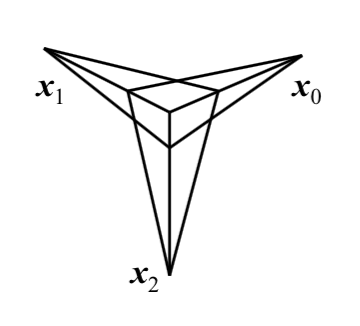
\includegraphics[width=0.4\textwidth]{figures/vanishing_points.png}
\end{center}
\caption{Visualisation of how the edges of a cuboid give rise to three orthogonal vanishing points.} % TODO hur referera? Tagen från szeliski s. 330
\label{fig:vanishing_points} % TODO bättre fig text, "beteckningar ska överensstämma.."
\end{figure}

The online configuration uses vanishing point calibration.
It is ideal to use vanishing point calibration for this particular problem since every cuboid package has three orthogonal sets of parallel lines which result in three orthogonal vanishing points.
Additionally, the known homography between the image plane and the top-plane of the package can be used to improve the estimate of $K$.

When the $K$ is known, the camera pose can be estimated as described in \ref{camera-pose}, using the four image-world point correspondences given by the reference object.
The method EPnP was chosen initially, but much better results were achieved with a regular, iterative approach. % TODO refer opencv?

Once the camera pose is obtained, equation \ref{eq:projection1} can be used, which means that any point in the world can be projected to a point in the image.
However, the reverse mapping is sought, i.e. the position of the package the world of the image coordinates of the bottom corners of the package, i.e. the reverse mapping.
This is generally not possible to do, unless something is known about the geometry of the scene.
Luckily, it is known that the lower corners share $X$, and $Y$ coordinates with a top corner, which position is already known.
The image coordinates $(u,v)$ of a lower corner, and the world coordinates $(X,Y)$ of the corresponding upper corner can then be used to solve for the $Z$ coordinate of the lower corner. 
Equation \ref{eq:projection3} can be transformed to the following over-defined system:
\begin{equation} \label{eq:constrained-projection}
\begin{pmatrix} up_{33}-p_{13} \\ vp_{33}-p_{23} \end{pmatrix} Z = 
\begin{pmatrix}
X(p_{11}-up_{31}) + Y(p_{12}-up_{32})+p_{14}-u \\
X(p_{21}-vp_{31}) + Y(p_{22}-vp_{32})+p_{24}-v
\end{pmatrix}
\end{equation}
This is solved as a least-squares problem using Single Value Decomposition (SVD).
Since two pairs of upper-lower corners which share $X$ and $Y$ coordinates are known, two least-squares solutions of $Z$ can be obtained.
The solution with the smallest error is chosen as $Z$.

\section{Evaluation} % TODO about the pictures, resolution, aspect ratio etc
To evaluate the performance of the detection and measuring algorithms two datasets were created.
One training dataset, used to optimise the many constants used by the algorithms, and one test dataset. % TODO how many constants? How is optimisation done?
The training dataset consisted of 50 images of five different packages.
The test dataset consisted of 225 images of five different packages.
The packages in the test dataset are shown in figure \ref{fig:packages}. A blue plastic folder was placed under the reference object on packages 3-5 to  add some contrast between the reference object and the white surfaces.

\begin{figure}
	\centering
	\begin{subfigure}[b]{0.3\textwidth}
		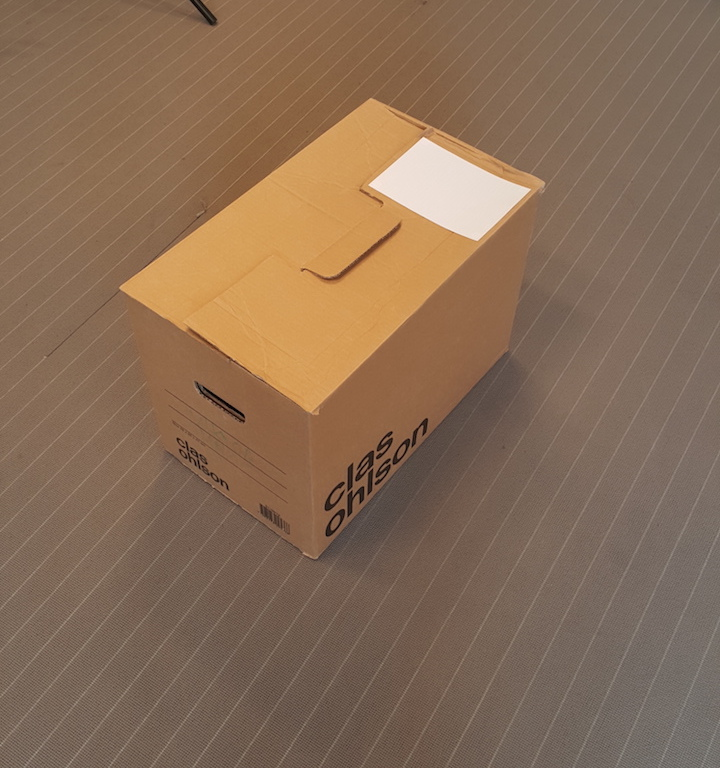
\includegraphics[width=\textwidth]{figures/package_1.jpg}
		\caption{}
		\label{fig:package_1}
	\end{subfigure}%
	~~~ %add desired spacing between images, e. g. ~, \quad, \qquad, \hfill etc.
	%(or a blank line to force the subfigure onto a new line)
	\begin{subfigure}[b]{0.3\textwidth}
		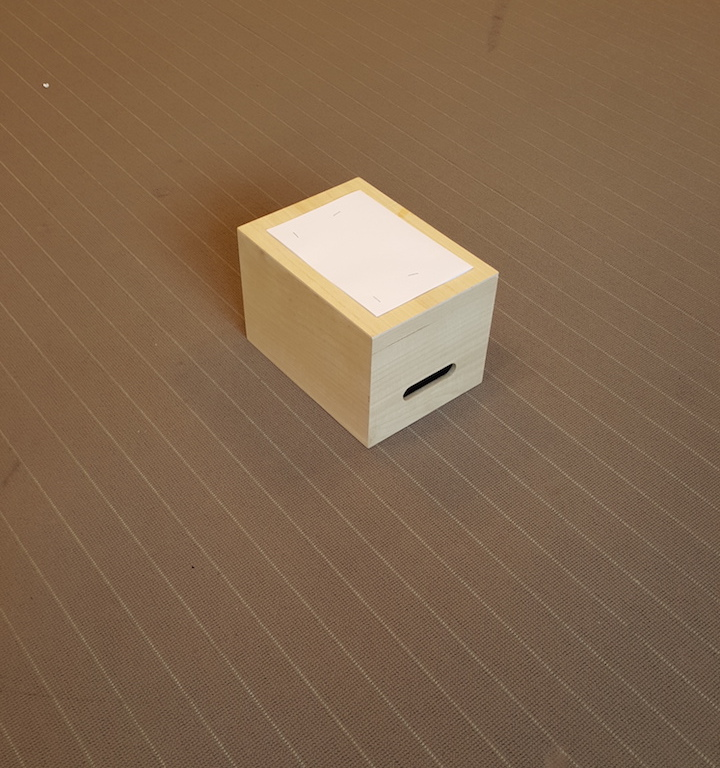
\includegraphics[width=\textwidth]{figures/package_2.jpg}
		\caption{}
		\label{fig:package_2}
	\end{subfigure}
	\vspace{3mm}\\
	\begin{subfigure}[b]{0.3\textwidth}
		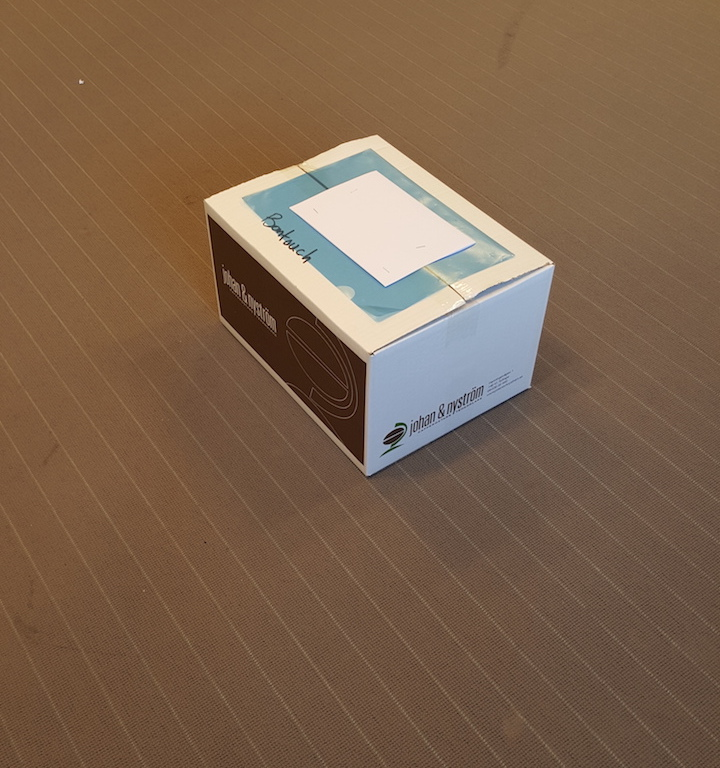
\includegraphics[width=\textwidth]{figures/package_3.jpg}
		\caption{}
		\label{fig:package_3}
	\end{subfigure}
	~~~
	\begin{subfigure}[b]{0.3\textwidth}
		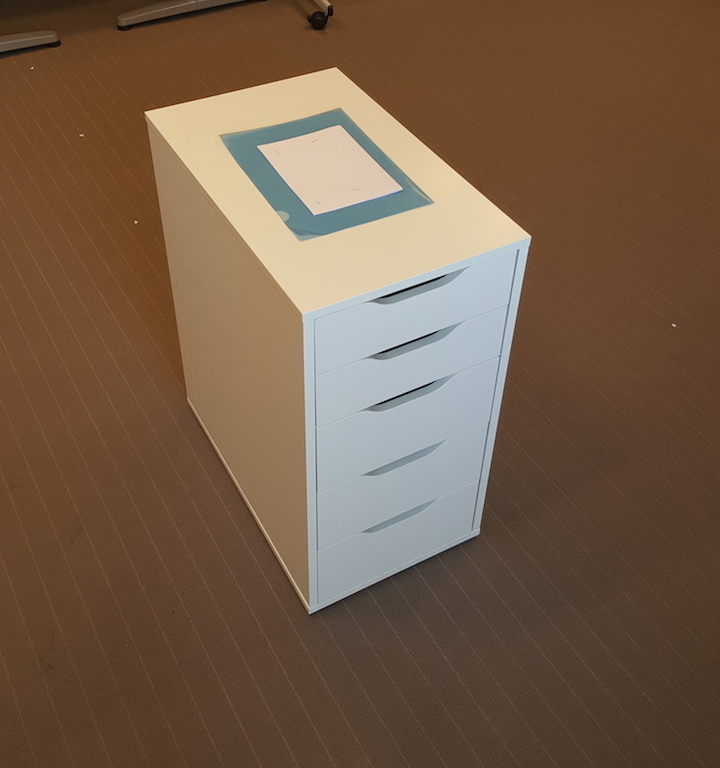
\includegraphics[width=\textwidth]{figures/package_4.jpg}
		\caption{}
		\label{fig:package_4}
	\end{subfigure}
	\vspace{3mm}\\
	\begin{subfigure}[b]{0.3\textwidth}
		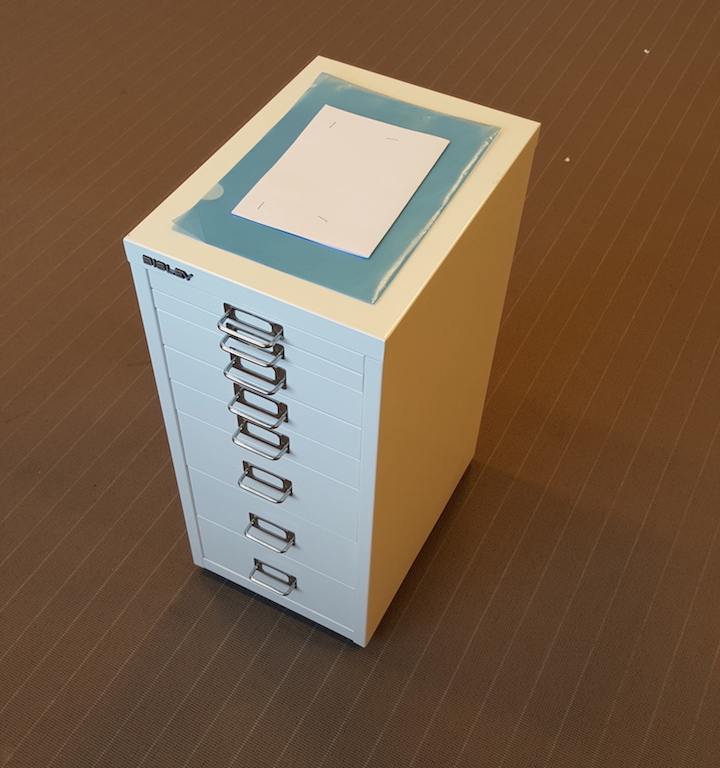
\includegraphics[width=\textwidth]{figures/package_5.jpg}
		\caption{}
		\label{fig:package_5}
	\end{subfigure}
	\caption[The packages in the test dataset]{The packages in the test dataset. (a) Package 1: A moving box ($580 \times 350 \times 405$ mm). (b) Package 2: A small wooden box ($260 \times 191 \times 177$ mm). (c) Package 3: A lightly textured cardboard box ($385 \times 295 \times 225$ mm). (d) Package 4: A white wooden filing cabinet ($580 \times 360 \times 690$ mm). (e) Package 5: A white metal filing cabinet ($383 \times 280 \times 605$ mm).}\label{fig:packages}
\end{figure}

The test dataset was constructed systematically with images observing the packages from different positions.
Three parameters were alternated: 
\begin{itemize}
	\item Distance to the centre of the package. 
			The used distances were 1, 1.5, and 2 metres.
	\item Height above the ground. 
			The used heights were 0.9, 1.2, and 1.5 metres for the first three packages, and 1.2, 1.5, and 1.8 metres for the latter two.
			The reason for the division is that the high height of the two latter packages made the viewing angle unreasonable when viewing them from 0.9 metres above ground, so the lowest height was removed, and a higher one added.
	\item Horizontal viewing angle. 
			Five different angles were used.
			Two were frontal views of the package, in which only two faces of the package could be observed. One of the longer side, and one of the shorter side.
			One image was taken between the two sides, with a $45^\circ$ angle to both sides.
			The last two images view the package with a sharp angle, about $15^\circ$ to the long or short side, respectively.
			An example from each position is shown in figure \ref{fig:positions}.
\end{itemize}

\begin{figure}
	\centering
	\begin{subfigure}[b]{0.2\textwidth}
		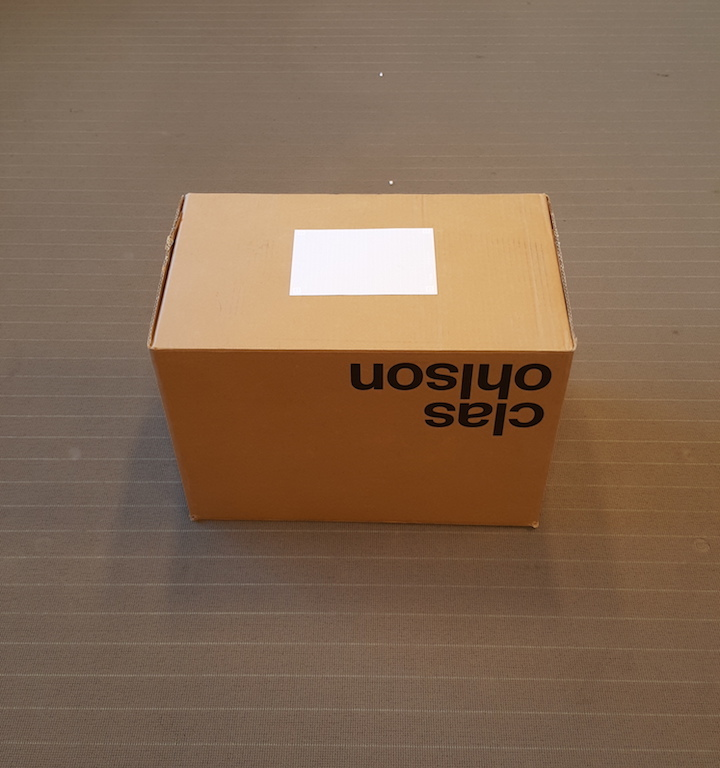
\includegraphics[width=\textwidth]{figures/angle_1.jpg}
		\label{fig:angle_1}
	\end{subfigure}
	~
	\begin{subfigure}[b]{0.2\textwidth}
		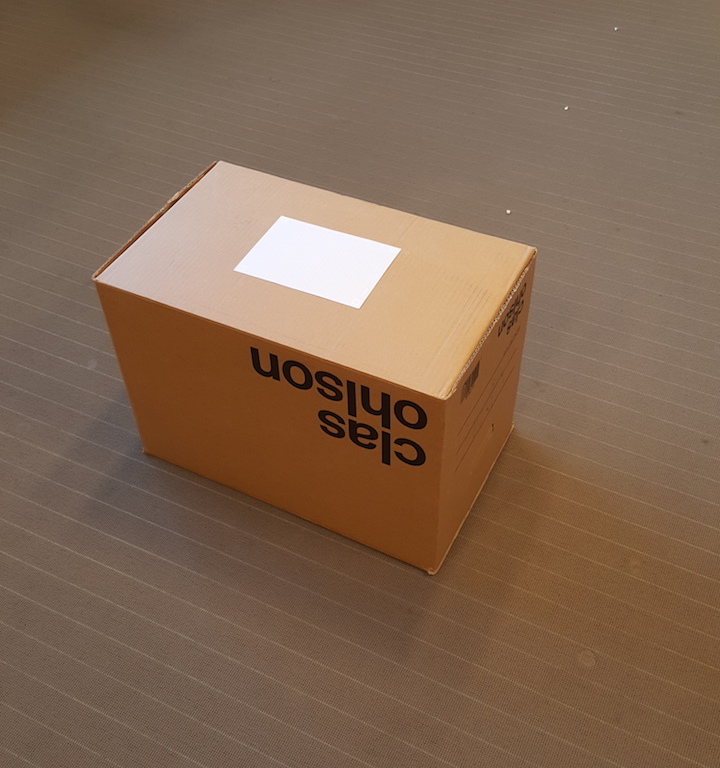
\includegraphics[width=\textwidth]{figures/angle_2.jpg}
		\label{fig:angle_2}
	\end{subfigure}
	~
	\begin{subfigure}[b]{0.2\textwidth}
		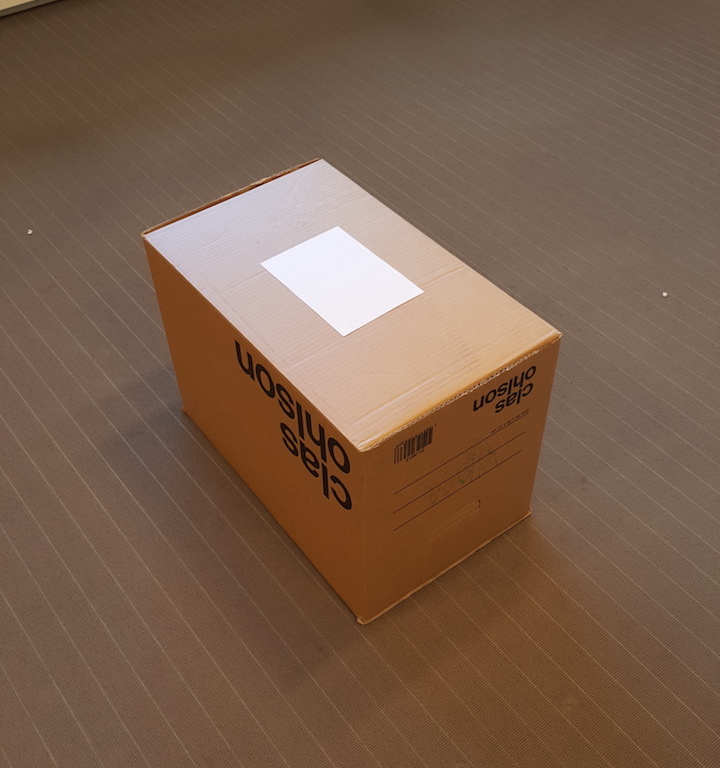
\includegraphics[width=\textwidth]{figures/angle_3.jpg}
		\label{fig:angle_3}
	\end{subfigure}
	
	\begin{subfigure}[b]{0.2\textwidth}
		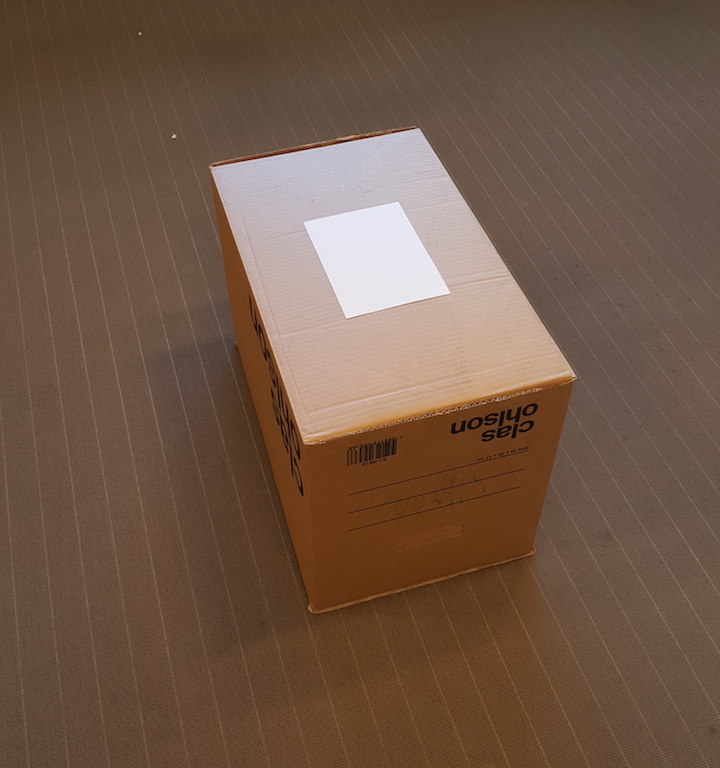
\includegraphics[width=\textwidth]{figures/angle_4.jpg}
		\label{fig:angle_4}
	\end{subfigure}
	~
	\begin{subfigure}[b]{0.2\textwidth}
		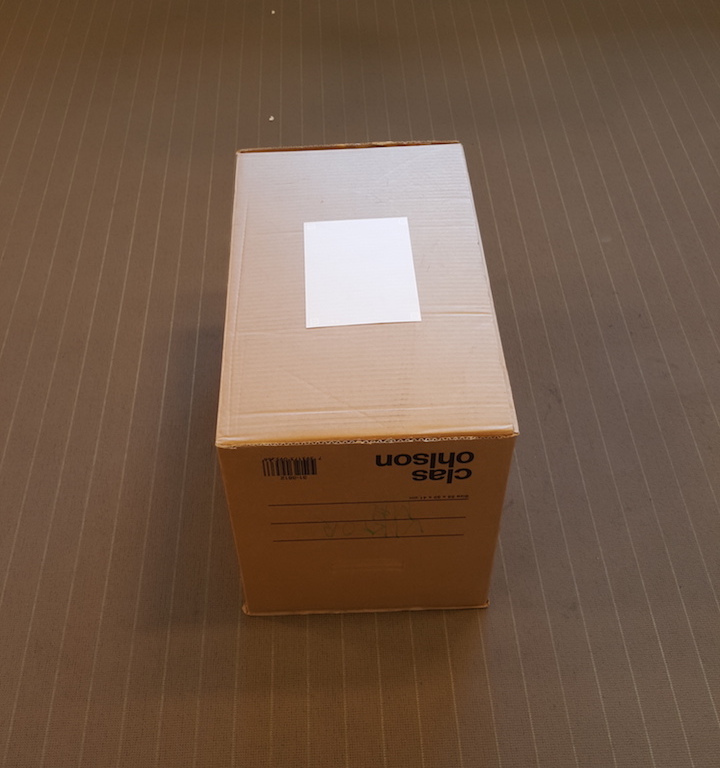
\includegraphics[width=\textwidth]{figures/angle_5.jpg}
		\label{fig:angle_5}
	\end{subfigure}
	\caption{Package 1 observed from the five different horizontal angles.}\label{fig:positions}
\end{figure}

All combinations of distances, heights, and horizontal angles resulted in 45 images per package.

\subsection{Benchmarking} \label{benchmarking}
A benchmarking program was constructed in order to measure the performance of the algorithms in the different cases.
The program ran the algorithms on each image, while gathering information about the success rates and accuracy.
The detection algorithm and measuring algorithm were tested both independently, and together, to show the performance of the individual pieces and of the whole system. 

The detection algorithm was tested by comparing the outputted corner points against ground truth locations of the reference object and package corners, which had been manually marked in each image.
The ability to detect the reference object, the package, and both in the same image, was tested.

The measuring algorithm was tested by using the ground truth locations as input, and comparing the resulting measurements against the ground truth dimensions of the package.
Both calibration methods, online vanishing point calibration, and offline calibration with Zhang's method, were tested.

The overall ability of the system was tested by running the whole algorithm and comparing the result with the ground truth dimensions of the package. 

%To simplify evaluation a test file (in JSON format) with information about each image was created.
%Each file contained information about which package was displayed in the image, the path to the image, the distance, height, and horizontal angle to the package, the dimensions of the package, and the locations of reference object and package corners in the image, which had been marked manually.

\subsection{Online testing} \label{method:online_testing}
A simple proof of concept Android application was made for online testing on the phone.
This was used to assert that it is feasible to run the algorithm on a smartphone.
Its purpose was also to determine if running the detection algorithm in real-time was an option.

The app simply displays the camera feed and continuously feeds new frames to the measuring algorithm.
When the package or reference object is successfully detected, an overlay is drawn to outline their position on the screen.
If both the package and reference are found in the same frame, the dimensions of the package are calculated, and each dimension is drawn next to the appropriate edge.
The processing time for each frame is also displayed.

The device used to run the test app is a Samsung Galaxy S6 Edge.
The S6 Edge was chosen because it currently tops benchmarks and tests, both regarding processing power and photo quality \cite{phone_performance_benchmark}\cite{phone_camera_benchmark}.
The S6 Edge was also used to capture the test images used for offline testing.











\chapter{Results} \label{results}
The results are divided into four parts.
In section \ref{results:detection} the results of detection are presented.
In section \ref{results:measuring} the results of measuring are presented.
In section \ref{results:overall} the results of detection and measuring combined are presented.
Finally, in section \ref{results:online} the results of online testing are presented.

\section{Detection} \label{results:detection}
The output of the detection algorithm was compared against ground truth positions of the reference object and package corners, as explained in section \ref{method:evaluation}.
The error was defined as the sum of distances between the detected points and actual points, divided by the length of the contour in the image.
A detection result was considered to be correct if the error was less than $10\%$.
This error metric was chosen to make the error invariant to resolution changes, and to make results comparable between different packages and distances.

Table \ref{table:detection_overall} shows the success rates and average relative error of detection.
It was clearly easier to detect the reference object than the package, but the package detection had a lower relative error.

\begin{table}%[H]
\centering
\begin{tabular}{@{} l *3c @{}}
\toprule
 & {Reference Object}  & {Package}  & {Reference Object and Package}  \\ 
\midrule
Success rate & 0.72 & 0.66 & 0.60 \\ 
Average error & 0.04 & 0.02 & \\
\bottomrule
 \end{tabular}
 \caption{Success rate and average error of detection.}
\label{table:detection_overall}
\end{table}

Table \ref{table:detection_categories} shows the success rates of detection grouped by four categories: package, rotation, distance, and height. Table \ref{table:detection_categories_error} shows the average relative error grouped in the same way.

\begin{table}[H]
\centering
\begin{tabular}{lcccc}
\toprule
\multicolumn{2}{c}{Category} & Reference Object & Package & Both\\
\midrule

\multirow{5}{*}{Package} 
& 1 & 0.73 & 0.49 & 0.47 \\ 
& 2 & 0.73 & 0.64 & 0.62 \\
& 3 & 0.78 & 0.93 & 0.76 \\
& 4 & 0.62 & 0.53 & 0.49 \\
& 5 & 0.71 & 0.69 & 0.67 \\
\midrule

\multirow{5}{1.5cm}{Horizontal angle}
& Long side		& 0.56 & 0.53 & 0.38 \\ 
& Angle long		& 0.73 & 0.78 & 0.69 \\
& Wide angle 		& 0.91 & 0.87 & 0.87 \\
& Angle short 	& 0.76 & 0.69 & 0.67 \\
& Short side		& 0.62 & 0.42 & 0.40 \\
\midrule
\multirow{3}{*}{Distance ($m$)} 
& 1 			& 0.56 & 0.53 & 0.38 \\ 
& 1.5  			& 0.73 & 0.78 & 0.69 \\
& 2 			& 0.91 & 0.87 &0.87 \\
\midrule
\multirow{3}{*}{Height} 
& Low 		& 0.51 & 0.44 & 0.37 \\ 
& Medium 	& 0.80 & 0.75 & 0.72 \\
& High		& 0.84 & 0.79 & 0.71 \\
\bottomrule
 \end{tabular}
 \caption{Success rate of detection by grouped by different categories.}
\label{table:detection_categories}
\end{table}


\begin{table}%[H]
\centering
\begin{tabular}{lccc}
\toprule
\multicolumn{2}{l}{Category} & Reference Object & Package\\
\midrule

\multirow{5}{*}{Package} 
& 1 & 0.04 & 0.02\\ 
& 2 & 0.04 & 0.03\\
& 3 & 0.04 & 0.03\\
& 4 & 0.04 & 0.01\\
& 5 & 0.04 & 0.03\\
\midrule

\multirow{5}{*}{Rotation}
& Frontal long		& 0.03 & 0.03 \\ 
& Sharp long	& 0.04 & 0.02 \\
& Wide angle 	& 0.04 & 0.02 \\
& Sharp short 	& 0.04 & 0.02 \\
& Frontal short	& 0.04 & 0.03 \\
\midrule
\multirow{3}{*}{Distance ($m$)} 
& 1 			& 0.03 & 0.02  \\ 
& 1.5  			& 0.04 & 0.02  \\
& 2 			& 0.05 & 0.03  \\
\midrule
\multirow{3}{*}{Height} 
& Low 		& 0.04 & 0.02 \\ 
& Medium 	& 0.04 & 0.02 \\
& High		& 0.04 & 0.02 \\
\bottomrule
 \end{tabular}
 \caption{Average relative error of detection by grouped by different categories.}
\label{table:detection_categories_error}
\end{table}


From table \ref{table:detection_categories} it can be concluded that the success rate of detection varied significantly between the entries in each category.
The frontal views yielded a much lower success rate than the other views.
The furthest distance and the lowest height also yielded lower success rates.
From table \ref{table:detection_categories_error} it can be concluded that the relative error did not vary much.
The error was consistently lower for the package than the reference object.

\section{Measuring} \label{results:measuring} 
Measuring results were obtained by using ground truth positions of the corners as input to the measuring algorithm, and comparing the output against the real dimensions of the packages.
The error was defined as the sum of the relative error of each dimension.
A measurement was considered to be correct if no dimension had a relative error greater than $10\%$.

Table \ref{table:measuring_overall} shows the success rate and average error of the two methods: uncalibrated views with vanishing point calibration, and calibrated views with Zhang's method.
It is shown that uncalibrated views had a lower success rate than calibrated views (81\% and 93\% respectively), but the average relative error was the same for both methods, 7\%.

\begin{table}%[H]
\centering
\begin{tabular}{@{} *3c @{}}
\toprule
&{Vanishing point calibration} & {Zhang's method}\\ 
\midrule
Success rate & 0.81 & 0.93 \\ 
Error & 0.07 & 0.07 \\
\bottomrule 
 \end{tabular}
 \caption{Success rate and average error of measuring.}
\label{table:measuring_overall}
\end{table} % TODO split error into x,y,z

Table \ref{table:measuring_categories} and \ref{table:measuring_categories_error} show the success rate and average error for the two methods, grouped by the same categories as in the previous section.

\begin{table}%[H]
\centering
\begin{tabular}{lccc}
\toprule
\multicolumn{2}{l}{Category} & Uncalibrated & Calibrated\\
\midrule

\multirow{5}{*}{Package} 
& 1 & 0.87 & 0.89 \\
& 2 & 0.84 & 0.98 \\
& 3 & 0.84 & 0.96 \\
& 4 & 0.71 & 1.00 \\
& 5 & 0.78 & 0.93 \\
\midrule

\multirow{5}{*}{Rotation}
& Frontal long		& 0.56 &  0.84 \\ 
& Sharp long		& 0.84 &  0.91 \\
& Wide angle 		& 0.98 &  0.98 \\
& Sharp short 		& 0.98 &  1.00 \\
& Frontal hort		& 0.69 &  0.93 \\
\midrule
\multirow{3}{*}{Distance ($m$)} 
& 1 			& 0.89 & 1.00   \\
& 1.5  			& 0.81 & 0.96   \\
& 2 			& 0.72 & 0.84   \\
\midrule
\multirow{3}{*}{Height} 
& Low 		& 0.80 & 0.87  \\
& Medium 	& 0.81 & 0.95  \\
& High		& 0.81 & 0.99  \\
\bottomrule
 \end{tabular}
 \caption{Success rate of measuring by grouped by different categories.}
\label{table:measuring_categories}
\end{table}

\begin{table}%[H]
\centering
\begin{tabular}{lccc}
\toprule
\multicolumn{2}{l}{Category} & Vanishing point calibration & Zhang's method\\
\midrule

\multirow{5}{*}{Package} 
& 1 & 0.09 & 0.08 \\
& 2 & 0.07 & 0.06 \\
& 3 & 0.07 & 0.06 \\
& 4 & 0.07 & 0.07 \\
& 5 & 0.05 & 0.06 \\
\midrule

\multirow{5}{*}{Rotation}
& Frontal long	& 0.08 & 0.08 \\\ 
& Sharp long	& 0.07 & 0.07 \\
& Wide angle 	& 0.07 & 0.07 \\
& Sharp short 	& 0.07 & 0.07 \\
& Frontal short	& 0.07 & 0.07 \\
\midrule
\multirow{3}{*}{Distance ($m$)} 
& 1 			& 0.07 & 0.06 \\
& 1.5  			& 0.07 & 0.07 \\
& 2 			& 0.08 & 0.08 \\
\midrule
\multirow{3}{*}{Height} 
& Low 		& 0.07 & 0.07 \\ 
& Medium 	& 0.07 & 0.07 \\
& High		& 0.07 & 0.07 \\
\bottomrule
 \end{tabular}
 \caption{Average error of measuring by grouped by different categories.}
\label{table:measuring_categories_error}
\end{table}


The results in table \ref{table:measuring_categories} are somewhat similar to the corresponding detection results.
The two frontal views yielded lower success rates, especially for vanishing point calibration.
Success rates also decreased as distance increased.
Table \ref{table:measuring_categories_error} shows very little change in average relative error.

\section{Overall performance} \label{results:overall}
The results in this section present the performance of the detection and measuring algorithms combined, using vanishing point calibration.
The errors are defined in the same way as in section \ref{results:measuring}.

Table \ref{table:overall_overall} shows the overall performance of detection and measuring combined.

\begin{table}%[H]
\centering
\begin{tabular}{@{} *2c @{}}
\toprule
 & {Overall performance}\\ 
\midrule
Success rate	& 0.51 \\ 
Error 			& 0.07 \\
\bottomrule 
 \end{tabular}
 \caption{Success rate and average error of detection and measuring combined.}
\label{table:overall_overall}
\end{table}

Table \ref{table:overall_categories} and \ref{table:overall_categories_error} show the success rate and average error of detection and measuring combined.

\begin{table}%[H]
\centering
\begin{tabular}{lcc}
\toprule
\multicolumn{2}{l}{Category} & Success rate\\
\midrule

\multirow{5}{*}{Package} 
& 1 & 0.40  \\
& 2 & 0.58  \\
& 3 & 0.62  \\
& 4 & 0.40  \\
& 5 & 0.56  \\
\midrule

\multirow{5}{*}{Rotation}
& Frontal long		& 0.18 \\ 
& Sharp long		& 0.64 \\
& Wide angle 		& 0.82 \\
& Sharp short 		& 0.62 \\
& Frontal hort		& 0.29 \\
\midrule
\multirow{3}{*}{Distance ($m$)} 
& 1 			& 0.57 \\
& 1.5  			& 0.64 \\
& 2 			& 0.32 \\
\midrule
\multirow{3}{*}{Height} 
& Low 		& 0.31 \\
& Medium 	& 0.67 \\
& High		& 0.56 \\
\bottomrule
 \end{tabular}
 \caption{Overall success rate by grouped by different categories.}
\label{table:overall_categories}
\end{table}

\begin{table}%[H]
\centering
\begin{tabular}{lcc}
\toprule
\multicolumn{2}{l}{Category} & Error\\
\midrule

\multirow{5}{*}{Package} 
& 1 & 0.08  \\
& 2 & 0.06  \\
& 3 & 0.06  \\
& 4 & 0.07  \\
& 5 & 0.07  \\
\midrule

\multirow{5}{*}{Rotation}
& Frontal long		& 0.08 \\ 
& Sharp long		& 0.08 \\
& Wide angle 		& 0.05 \\
& Sharp short 		& 0.07 \\
& Frontal hort		& 0.10 \\
\midrule
\multirow{3}{*}{Distance ($m$)} 
& 1 			& 0.07 \\
& 1.5  			& 0.07 \\
& 2 			& 0.08 \\
\midrule
\multirow{3}{*}{Height} 
& Low 		& 0.08 \\
& Medium 	& 0.07 \\
& High		& 0.07 \\
\bottomrule
 \end{tabular}
 \caption{Overall error by grouped by different categories.}
\label{table:overall_categories_error}
\end{table}

The results are similar to those of the individual parts, as can be expected.
The lower success rates of the frontal views, the furthest distance and the lowest height, are even more prominent in this case.
The average relative errors vary slightly more than for the individual parts.

It is obvious that the poor performance of certain positions drags down the overall success rate significantly.
It is therefore of interest to see the results of only the "good positions".
Table \ref{table:overall_good} shows the overall performance of the system if the poorly performing positions are disregarded, i.e. the frontal views, the furthest distance, and the lowest height.

\begin{table}%[H]
\centering
\begin{tabular}{@{} *2c @{}}
\toprule
 & {Overall performance}\\ 
\midrule
Success rate	& 0.92 \\ 
Error 			& 0.06 \\
\bottomrule 
 \end{tabular}
 \caption[Improved overall success rate and average error of the system, when some positions are disregarded]{Success rate and average error of detection and measuring combined, while disregarding the poorly performing positions. The disregarded positions are the frontal views, where only two sides of the package can be seen, the furthest distance (2 metres), and the lowest height (0.9 or 1.1 metres). }
\label{table:overall_good}
\end{table}

Table \ref{table:overall_good} shows that disregarding a few of the positions resulted in a considerably better performance.
After disregarding the poorly performing positions, 60 images of the original 225 remained.

\section{Online testing} \label{results:online}

Online testing was performed using the Android application described in \ref{method:online_testing}.
A screenshot of the resulting application is shown in figure \ref{fig:screenshot}. % TODO add more screenshots?
The processing time of the application was typically around 300 milliseconds at the resolution $800 \times 450$ pixels on the Galaxy S6 Edge, depending on the amount of clutter in the image. 
More clutter resulted in higher processing times.

As previously described the application continuously sends image frames from the camera to the measuring algorithm. 
When the algorithm has finished, an overlay with the detected corner points and measurements are drawn on top of the camera feed.
With processing times of around 300 milliseconds the overlay would easily get misplaced in between frames if one was not careful to hold the camera still. 

The online testing was not performed in a very formal manner, since the purpose was only to confirm that it is feasible to run the algorithm on a modern smartphone, not to accurately measure processing times.

\begin{figure}%[H]
\begin{center}
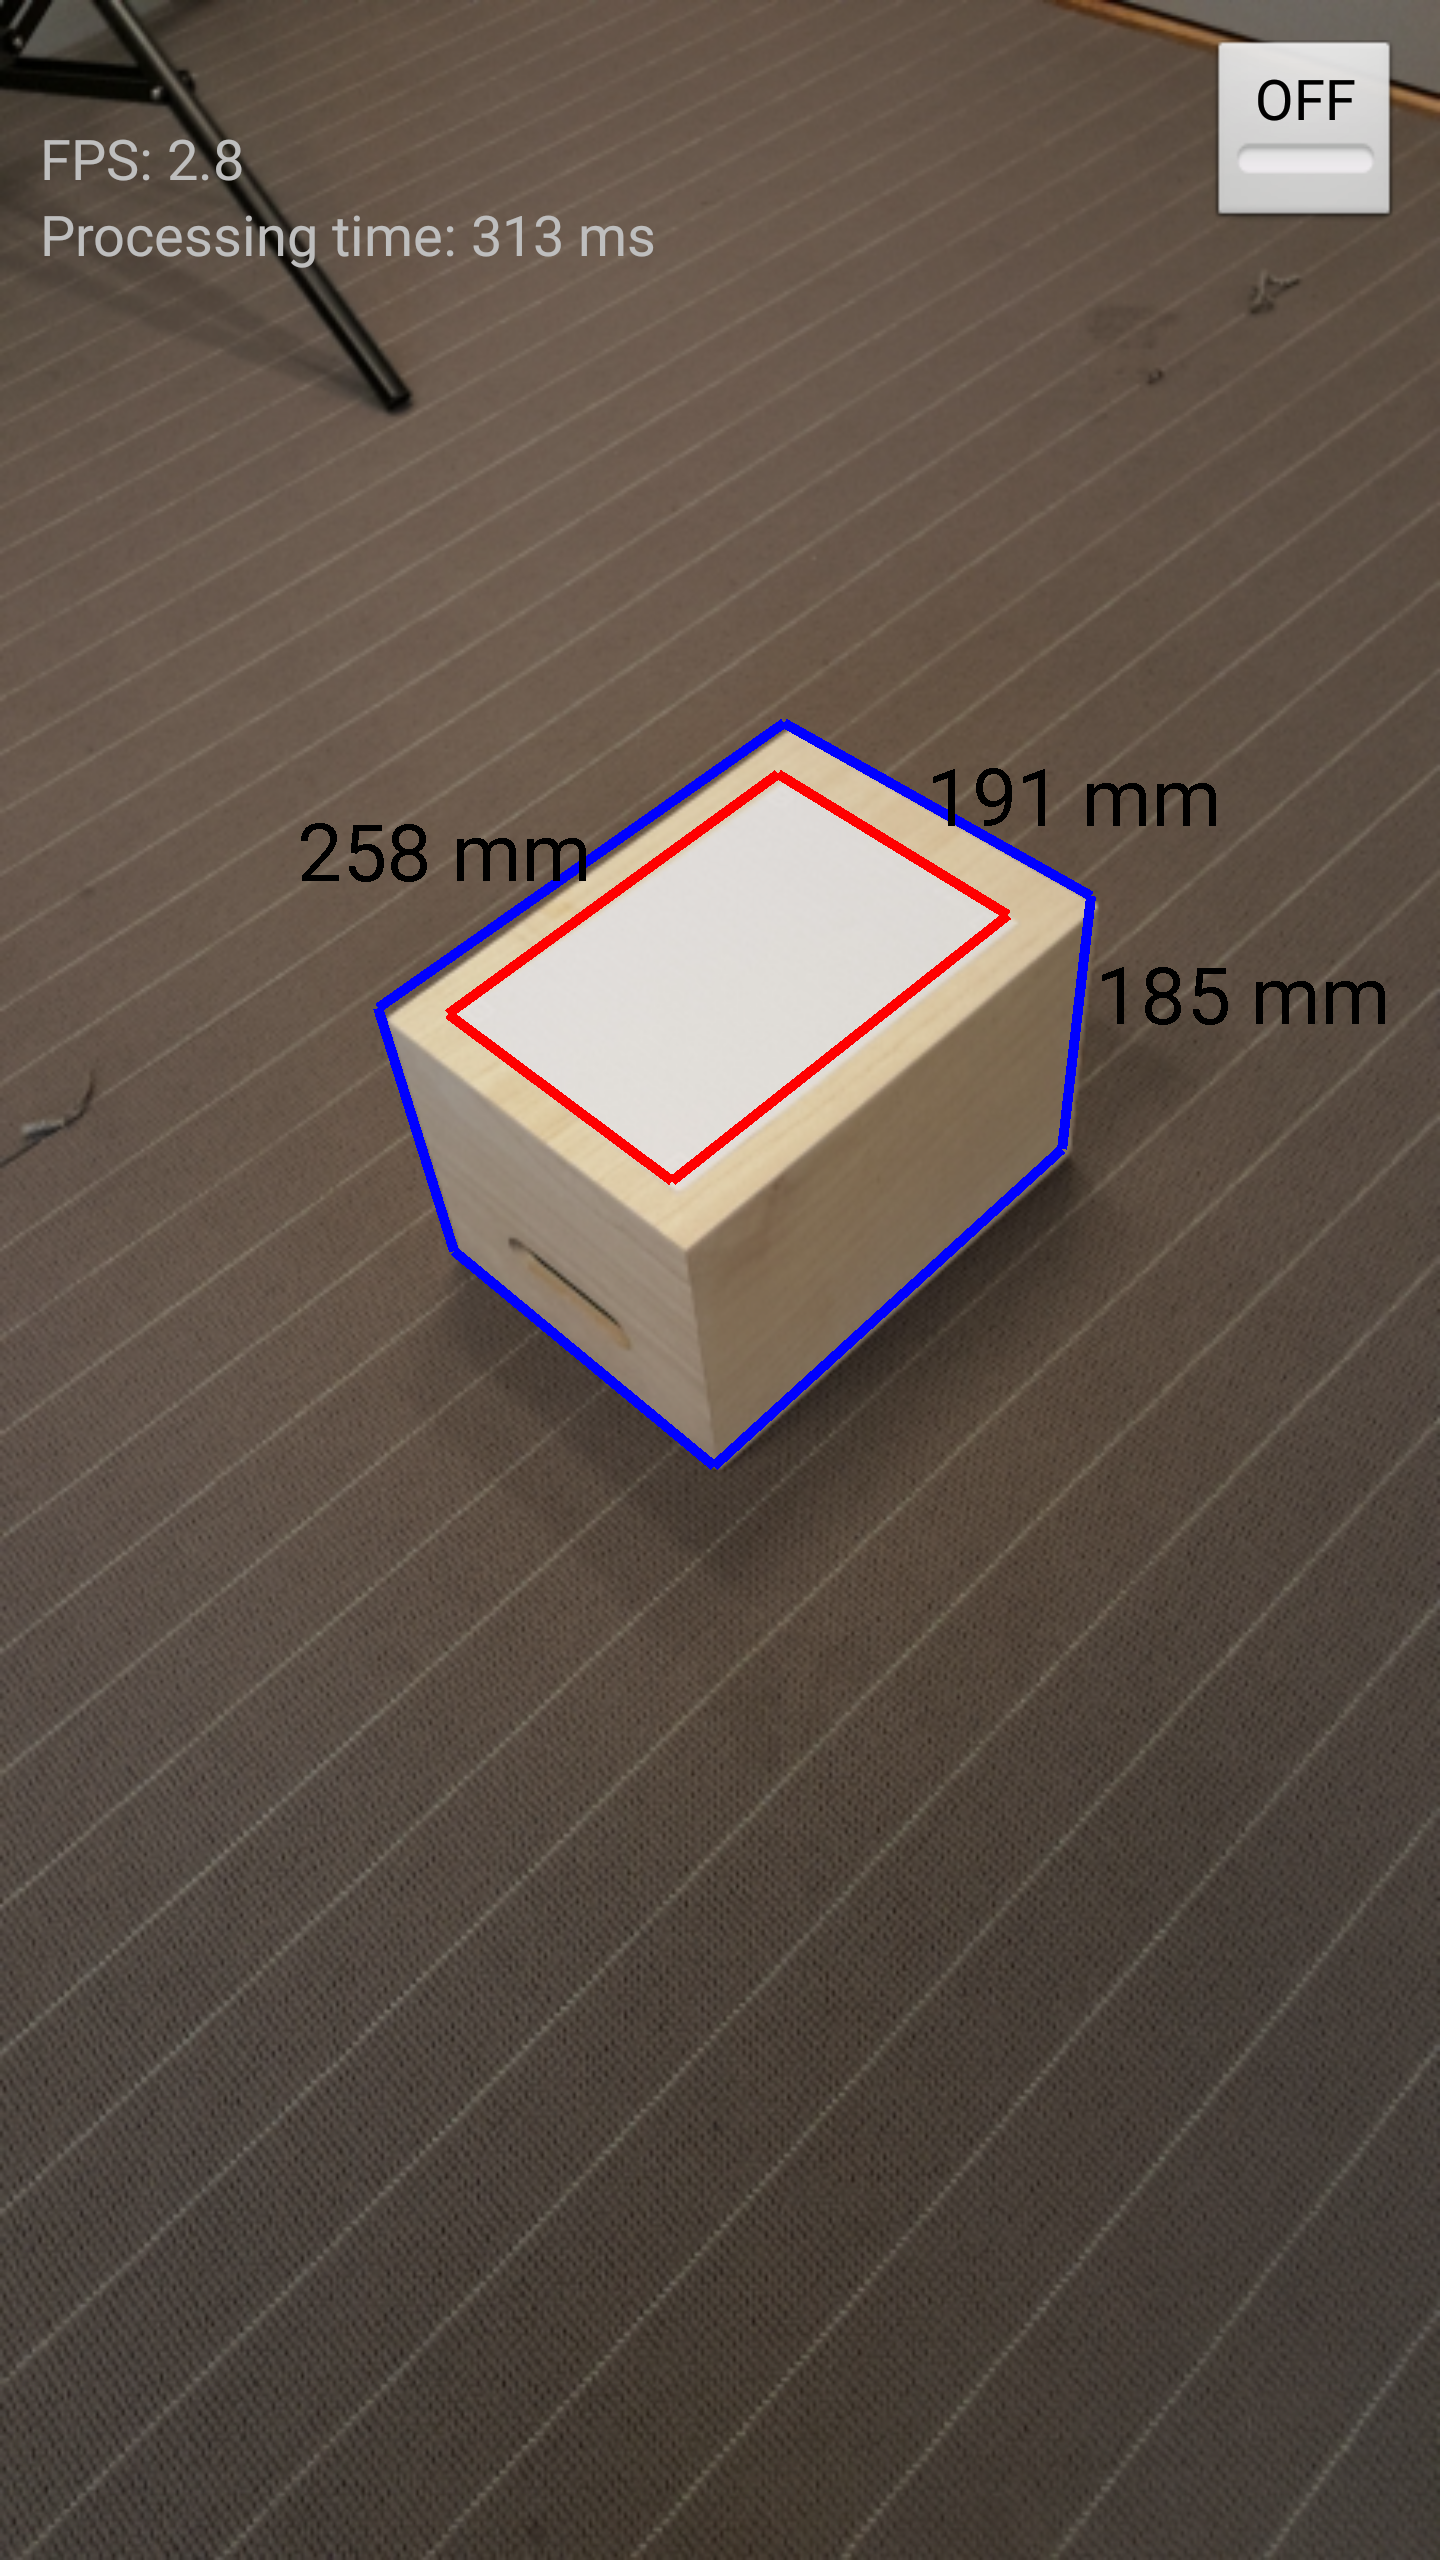
\includegraphics[width=0.6\textwidth]{figures/screenshot.png}
\end{center}
\caption{Screenshot of the app measuring package 2. A blue outline has been drawn around the package, and a red outline has been drawn around the reference object. The resulting dimensions are $258 \times 191 \times 185$ mm. The real dimensions of the package are $260 \times 191 \times 177$ mm.}
\label{fig:screenshot}
\end{figure}

\chapter{Discussion}
The results showed that the used method works well when using images of a package being observed from an angle where three faces of the package are visible, and at sufficiently close range and high altitude. 
As shown in table \ref{table:overall_good}, the success rate increased from 51\% to 92\% when selecting a subset of the camera poses.
The average error was also reduced from 7\% to 6\%.
The results from the selected subset of camera poses are satisfying, and suggestions on how to improve the performance of the remaining cases will be proposed.

Aside from success rates, this method performs the measurements of cuboids automatically, entirely without user intervention.
Additionally, no prior calibration, or special calibration objects are required.
That is avoided by using the fact that the package acts as a calibration object.
The only additional required object except for the package is a reference object.
In the current implementation, only white papers are detected, but detection of other planar objects, like credit cards for example, can easily be added.
A different planar reference object can be used directly by the measuring algorithm, the only requirement is that it must fit on top of the package.
With a small modification it could be placed on the floor next to the package instead.

\section{Detection} \label{discussion:detection}
The detection algorithm was based on simple, model-based method. 
The method involved detecting lines in the image and attempting to match the intersections between lines to a quadrilateral or hexagon in which opposing sides have as equal length, and are as parallel as possible.

The image processing algorithms used by this method depend on several constants.
Finding good values for the constants is critical.
They can not be too strict, because then important features can sometimes be left out, but they can not be too tolerant either, because then too much unimportant data can be left in the image, so that it is difficult to make sense of the data, or it takes too long to process.
For this task, is seemed impossible to choose a single value for a constant which yielded good enough data every time.
Many examples where there was too much, or too little data left to analyse for the paper or package detection algorithms exist in the test dataset.
This balance was extra important in this case, since the algorithm is supposed to be run on a smartphone with with limited processing power and with limited processing time.
This was one of the most common reasons of failure for the detection algorithms.

The tables in section \ref{results:detection} showed that the detection algorithm was much more successful for images taken from certain positions.
These were the three rotations from which three faces of the package could be seen, the two closest distances, and the two highest heights.
Regarding the rotations, it is believed that the variations are exclusively because the constraints and rules imposed by the algorithm, were better suited for three face views, than two faced views.
Initially, the algorithm was only designed with three face views in mind.

Regarding the variations in success rate connected to distance and height, it is believed to be partly because of implementation details and threshold values which favoured the higher and closer configurations, but they are also more difficult by nature.
As height increases, less clutter is seen in the background, and more of the floor.
As distance increases, there is room for more clutter in the background.
When there is more clutter, it is more difficult to distinguish what is truly relevant in the image, and it is more likely that there are too many lines.

%The scoring function was also not always good enough.
%In some cases there was another hexagon with opposing edges more parallel and with more similar length than the package.
%Some other criteria were considered, but sadly there was not enough time to implement them.
%For example additional score could be awarded if the inner contours of the package are detected.
%Currently, the inner contours of the package are filtered out, to reduce the amount of data.
%This addition would require them to be kept, which would in turn call for more intelligent pruning of edges as packages sometimes have a lot of texture which can make the amount of data overwhelming.
%
%Another reason for the poor performance of two-face views is that as distance grows, the edges going from bottom to the middle and from the middle to the top of the package contour, become increasingly parallel. 
%If the picture is not taken precisely in front of the middle of the package, but slightly towards the right or the left, the two edges can become inseparable.

% TODO additional reasons:
% from some angles the constraints imposed by the detection algorithm causes detection to fail (?)
% sometimes packages fail because they are not straight enough (?)

%In the current implementation only a tiny bit of an edge must be detected for it to be used as a potential package edge, since it is often the case that the full package contour cannot be found.
%It is not modelled that a candidate with detected edges along much of its contour is more likely to be the package.
%This could help with nonsensical candidate sometimes winning.

\section{Measuring}
The tables in section \ref{results:measuring} showed that vanishing point calibration failed more often than when using Zhang's method, but the accuracy was the same between the two methods.
It is somewhat surprising that there was no significant difference in accuracy among the accepted measurements.
A drop in success rate from $93\%$ to $81\%$ seems like a very reasonable sacrifice to make to gain the practicality of using uncalibrated views.
From a commercial perspective, it would be unfeasible to ask the users of a smartphone application to perform the calibration procedure.
Therefore it is very good news that the uncalibrated method worked so well.

Two main reasons were found to cause the lower success rate of vanishing point calibration: infinite vanishing points, and increased vulnerability to errors in detection.

Infinite vanishing points occur when the parallel lines of the package are parallel in the image as well, and hence do not result in a finite vanishing point. 
If an infinite vanishing point does occur, a constraint on $\omega$ is lost.
However, since the system is overdetermined, the calibration should still work in theory, even with up to two infinite vanishing points, if the vanishing point in the $Z$-direction is not one of the infinite ones, in which case the calibration becomes degenerate.
In practice the error was often too great, when one vanishing point was infinite. 
An infinite vanishing point occurred in 13 images in the test set, and in only one of these cases, a correct answer was found.
Infinite vanishing points only occurred with frontal view images, which also explains the greater difference in success rate between two and three face views, when using vanishing point calibration, compared to Zhang's method.

The vanishing point calibration method was also more vulnerable to errors in the package corners, since both the calibration and measurements themselves depend on the location of the package corners being correct.

%Errors do not necessarily increase proportionally with the error 
% TODO find out correlation between error in detection and measurement! 

%Due to the inaccuracies a different solution than the correct one have smaller least squares error than the correct answer, is therefore chosen as the solution.
%These problem occur when using detected corner points as well as when using the marked corners, since the marked corners also have some error.
%On average, the accepted solutions have the same error when using detected corner points and marked corners. % TODO förtydliga hur marked corners går till i metod
\section{Online testing} % TODO measure average processing time properly and show in results?
Online testing showed that the used method works well on a smartphone as well.
With a processing time of about 300 ms on the resolution $800 \times 450$, it is not yet quite fast enough to deliver a good user experience when used in real-time, at least not using the created demo application.
Unless one was very careful to hold the camera still, the overlay would move off the edges of the package, since the rate at which the overlay is updated is much slower than the rate at which new camera frames are displayed.
However, the algorithm could, in its current state, provide satisfying results in a non-real time application.
Such an application could for example let the user take one, or a few snapshots, process the snapshots, and display the result in a still image, instead of drawing the overlay on the live camera feed.

\section{Limitations}									
There are some limitations as to what the results can show, as a consequence of limitations in the evaluation method.
For example only one room was used for testing.
It was not an optimal environment, due to the striped floor and suboptimal lighting conditions.
The colour of the floor was also quite similar to the colour of one of package 1, which caused some issues.
However, performance is not guaranteed to be the same in other environments.

Another limitation is that not much effort was put into dealing with false positives.
The only countermeasure to this is that minimum score thresholds where added to the rating algorithm, i.e. a reference object or package hypothesis with a too low score were discarded even if it was the best hypothesis.

\section{Future work} \label{discussion:future_work}
It is clear from the results that the detection is currently the bottleneck of the algorithm.
Some suggestions on how to improve the detection algorithm on a high level were presented in section \ref{discussion:detection}, but the lower level image processing algorithms can also be improved.
An improvement with much potential is to fix the problem of using constant thresholds for the image processing algorithms.
One can use thresholding techniques to automatically determine good thresholds to detect edges in an image, or a region of an image.
This can be done in conjunction with Canny edge detection, as shown in \cite{wang2005fast} and \cite{liu2004automated}.
This would also improve the chances of the algorithm working in different environments.

Alternatively, a completely different approach could be used for object detection, such as the one presented in "Localizing 3D cuboids in single-view images" as mentioned in section \ref{related_work:object_detection}.
This method can handle different poses well, occlusion, and clutter.
However, it is unclear if this method is feasible to use, given the processing time constraints.

Another interesting improvement is to use multiple images to measure the package.
One could either use multiple measurements and simply calculate an average, combined with outlier rejection with for example RANSAC \cite{fischler1981random}.
This should both improve success rate and accuracy.
In the same way, one could save the intrinsic matrices found with vanishing point calibration between measurements and combine them.
They should then converge over time to a very accurate calibration matrix. 

% Nämn object tracking och rois. \cite{yilmaz2006object}

\section{Conclusions}
A method to measure the dimensions of cuboid packages using a single, uncalibrated view, has been presented.
The algorithm could successfully measure the package in $51\%$ of all images in the test set, which consisted of 225 images of 5 packages from various positions.
However, the algorithm could handle some of the camera poses much better than others.
If only a subset of the camera poses were chosen, a success rate of $92\%$ was achieved instead.
The images in the subset were those where three faces of the package could be seen, those taken from the two closer of the distances (1 and 1.5 metres), and those taken from the two of the higher heights (1.2 and 1.5, or 1.5 and 1.8 metres).
The difference in performance largely depended on implementation details, but problems such as increased clutter and infinite vanishing points occurred in the poorly performing positions, also factored in.

A version of the algorithm which used calibrated views was also implemented, to determine how much performance needed to be sacrificed to gain the convenience of not having to go through the calibration procedure.
The success rates when testing the measuring algorithm in isolation was $81\%$ for uncalibrated views, and $93\%$ for calibrated views.
The average relative error was $7\%$ for both methods.

Online testing showed that the algorithm is not yet mature to be run in a real-time application, but could work well in a non-real time application.

% TODO bättre resultat om man skulle constraina mer, t.ex. tvinga paketet att va i en fyrkant i centrum av bilden.
% TODO comment on results by package

% TODO mention classification of 2d vs 3d view

% TODO för att förbättra nogrannhet, använd fler vps




%----------------------------------------------------------------------------------------
%	BIBLIOGRAPHY
%----------------------------------------------------------------------------------------

\bibliographystyle{unsrt}
\bibliography{references}

%----------------------------------------------------------------------------------------
%	APPENDIX
%----------------------------------------------------------------------------------------
%\appendix
%\addappheadtotoc
%\chapter{An appendix}\label{appA}
%that we refer to here: \ref{RDF_4}

\end{document}
